\documentclass[11pt]{article}
\usepackage{amssymb}
\usepackage{amsthm}
\usepackage{enumitem}
\usepackage{physics,amsmath}
\usepackage{bm}
\usepackage{adjustbox}
\usepackage{mathrsfs}
\usepackage{graphicx}
\usepackage{siunitx}
\usepackage[mathscr]{euscript}

\title{\textbf{Solved selected problems of Classical Mechanics - Gregory}}
\author{Franco Zacco}
\date{}

\addtolength{\topmargin}{-3cm}
\addtolength{\textheight}{3cm}

\newcommand{\hatr}{\bm{\hat{r}}}
\newcommand{\hatx}{\bm{\hat{x}}}
\newcommand{\haty}{\bm{\hat{y}}}
\newcommand{\hatz}{\bm{\hat{z}}}
\newcommand{\hatn}{\bm{\hat{n}}}
\newcommand{\hati}{\bm{\hat{i}}}
\newcommand{\hatj}{\bm{\hat{j}}}
\newcommand{\hatk}{\bm{\hat{k}}}
\newcommand{\uvi}{\bm{i}}
\newcommand{\uvj}{\bm{j}}
\newcommand{\uvk}{\bm{k}}
\newcommand{\hatth}{\bm{\hat{\theta}}}
\newcommand{\hatphi}{\bm{\hat{\phi}}}
\newcommand{\hatrho}{\bm{\hat{\rho}}}
\newcommand{\ngrad}[1]{\text{grad}_{\bm{#1}}}

\theoremstyle{definition}
\newtheorem*{solution*}{Solution}
\renewcommand*{\proofname}{\bf{Solution}}

\begin{document}
\maketitle
\thispagestyle{empty}

\section*{Chapter 19 - Problems in rigid body dynamics}

\begin{proof}{\textbf{19.1}}
    Let us consider the following system
    \begin{center}
        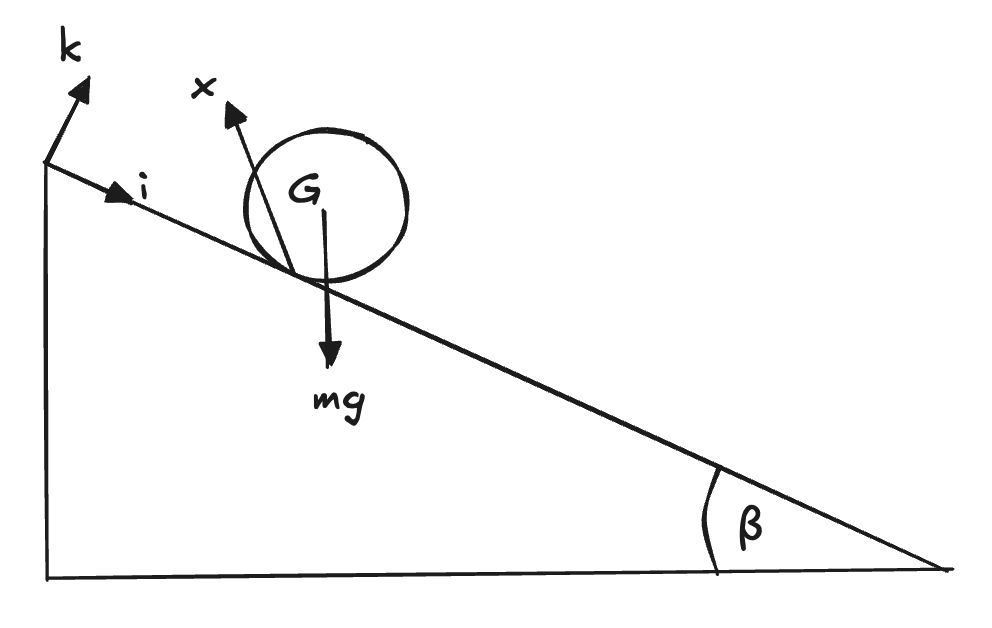
\includegraphics[scale=0.3]{ch19-1.png}
    \end{center}
    Then from the governing equations we have that
    \begin{align*}
        m\bm{\dot{V}} &= \bm{X} + mg\sin\beta\bm{i} - mg\cos\beta\bm{k}\\
        \bm{\dot{L}}_G &= (-b\bm{k}) \times \bm{X} 
    \end{align*}
    Where $\bm{X}$ is the reaction of the table exerted on the ball.
    Using that $\bm{L}_G = A\bm{\omega}$ and eliminating the reaction $\bm{X}$
    we get that
    \begin{align*}
        A\bm{\dot{\omega}}
        &= (-b\bm{k})
        \times (m\bm{\dot{V}} - mg\sin\beta\bm{i} + mg\cos\beta\bm{k})\\
        &= b(m\bm{\dot{V}} - mg\sin\beta\bm{i} + mg\cos\beta\bm{k})
        \times \bm{k}\\
        &= mb\bm{\dot{V}}\times\bm{k} - mgb\sin\beta\bm{i}\times \bm{k}\\
        &= mb\bm{\dot{V}}\times\bm{k} + mgb\sin\beta\bm{j}
    \end{align*}
    On integrating with respect to $t$ we get that
    \begin{align*}
        A\bm{\omega} + mb\bm{k}\times\bm{V} &= \bm{C} + mgbt\sin\beta\bm{j}
    \end{align*}
    Where $\bm{C}$ is a constant vector. In particular if we take the scalar
    product of this equation with $\bm{k}$, we have that
    \begin{align*}
        A\bm{\omega}\cdot\uvk + mb(\bm{k}\times\bm{V})\cdot\uvk
        &= \bm{C}\cdot\uvk + mgbt\sin\beta\bm{j}\cdot\uvk\\
        A\bm{\omega}\cdot\uvk &= n
    \end{align*}
    Where $n$ is a constant. Also, we used that $\uvj \cdot \uvk = 0$ and 
    the triple product is also 0. Therefore we see that the component of
    $\bm\omega$ in the direction of $\uvk$ (perpendicular to the inclined
    plane) is constant independent of the motion of the ball.

    If we now consider that the ball is rolling, then the particle $C$ in
    contact with the plane has zero velocity, so the rolling condition give us
    \begin{align*}
        \bm{V} + b\uvk \times \bm{\omega} = \bm{0}
    \end{align*}
    Now, by cross-multiplying the conservation principle by $\uvk$ we have that 
    \begin{align*}
        A\uvk \times \bm{\omega}
        &= \uvk \times \bm{C} + mgbt\sin\beta\uvk\times\uvj
        - mb\uvk \times(\bm{k}\times\bm{V})\\
        &= \uvk \times \bm{C} - mgbt\sin\beta\uvi
        - mb((\uvk\cdot\bm{V})\uvk - (\uvk\cdot\uvk)\bm{V})\\
        &= \uvk \times \bm{C} - mgbt\sin\beta\uvi + mb\bm{V}
    \end{align*}
    Therefore by joining this equation and the rolling condition equation
    we get that 
    \begin{align*}
        \bm{V} + \frac{mb^2}{A}\bm{V}
        &= -\frac{b}{a}\uvk \times \bm{C} + mgbt\sin\beta\uvi\\
        \bm{V} + \frac{mb^2}{A}\bm{V}
        &= \frac{b}{a}\bm{C}\times\uvk + mgbt\sin\beta\uvi
    \end{align*}
    This shows that $\bm{V}$ is dependent on time. If
    we integrate again this equation we see that the rolling motion
    depends on $t^2$ and therefore the path of the ball must be a parabola.  
\end{proof}
\cleardoublepage
\begin{proof}{\textbf{19.2}}
    Let us consider the following system
    \begin{center}
        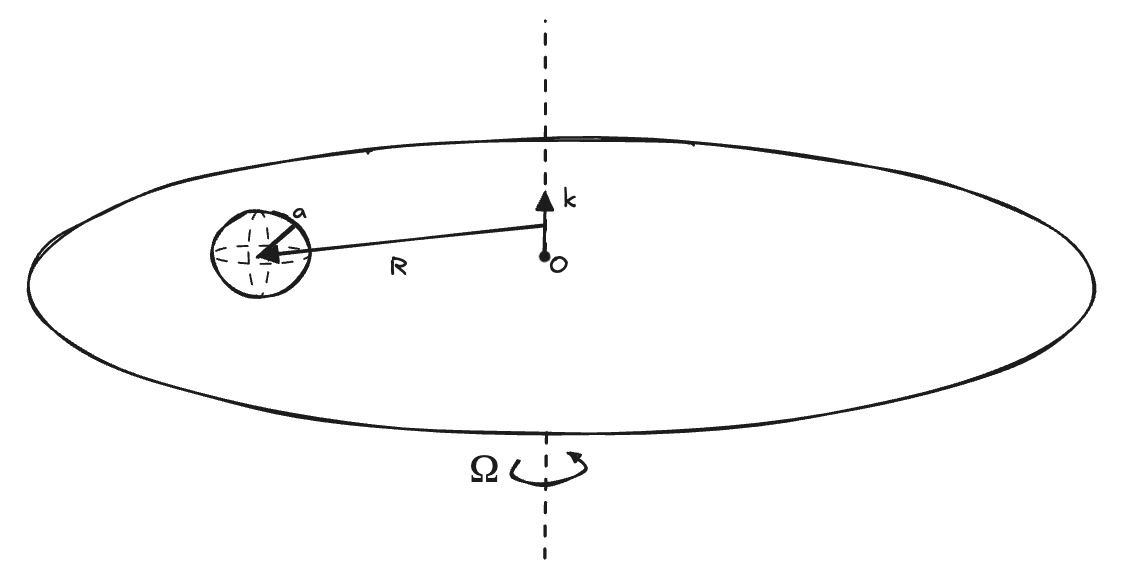
\includegraphics[scale=0.3]{ch19-2.png}
    \end{center}
    Then from the governing equations we have that
    \begin{align*}
        m\bm{\dot{V}} &= \bm{X} - mg\bm{k}\\
        \bm{\dot{L}}_G &= (-a\bm{k}) \times \bm{X} 
    \end{align*}
    Where $\bm{X}$ is the reaction of the turntable exerted on the ball.
    Using that $\bm{L}_G = A\bm{\omega}$ where $A = \frac{2}{5}ma^2$ is the
    moment of inertia of the ball, then eliminating the reaction $\bm{X}$
    we get that
    \begin{align*}
        A\bm{\dot{\omega}}
        &= (-a\bm{k})
        \times (m\bm{\dot{V}} + mg\bm{k})\\
        &= a(m\bm{\dot{V}} + mg\uvk)
        \times \bm{k}\\
        &= ma\bm{\dot{V}}\times\bm{k}
    \end{align*}
    On integrating with respect to $t$ we get that
    \begin{align*}
        A\bm{\omega} + ma\bm{k}\times\bm{V} &= \bm{C}
    \end{align*}
    Where $\bm{C}$ is a constant vector. In particular if we take the scalar
    product of this equation with $\bm{k}$, we have that
    \begin{align*}
        A\bm{\omega}\cdot\uvk + ma(\bm{k}\times\bm{V})\cdot\uvk
        &= \bm{C}\cdot\uvk\\
        A\bm{\omega}\cdot\uvk &= n
    \end{align*}
    Where $n$ is a constant. Also, we used that the triple product is also 0.
    Therefore we see that in any motion of the ball, the vertical spin
    $\bm{\omega}\cdot\uvk$ is constant.

    If we now consider that the ball is rolling, then the particle $C$ in
    contact with the turntable has zero velocity, so the rolling condition give
    us
    \begin{align*}
        \bm{V}_C = \bm{V} + a\uvk \times \bm{\omega} = \bm{0}
    \end{align*}
    Also, from the equation for $A \bm{\dot\omega}$ we derived above, replacing
    the value of $A$ we have that
    \begin{align*}
        \frac{2}{5}ma^2\bm{\dot{\omega}}
        &= ma\bm{\dot{V}}\times\bm{k}\\
        \frac{2}{5}a\bm{\dot{\omega}}
        &= \bm{\dot{V}}\times\bm{k}
    \end{align*}
    And cross-multiplying this equiation by $\uvk$ we obtain an expression for
    $\bm{\dot V}$ as follows
    \begin{align*}
        \frac{2}{5}a\uvk \times \bm{\dot{\omega}}
        &= \uvk \times(\bm{\dot{V}}\times\bm{k})\\
        \frac{2}{5}a\uvk \times \bm{\dot{\omega}}
        &= \bm{\dot{V}} (\uvk\cdot\uvk) - \uvk(\uvk\cdot\bm{\dot{V}})\\
        \frac{2}{5}a\uvk \times \bm{\dot{\omega}}
        &= \bm{\dot{V}}
    \end{align*}
    If we assume the position of the ball's center of mass is determined by a
    vector $\bm{R}$ from the axis $\{O, \uvk\}$ then the velocity $\bm V_C$
    of the particle $C$ is also
    \begin{align*}
        \bm{V}_C = \Omega\uvk \times \bm{R}
    \end{align*}
    Hence by joining the rolling condition and this equation we have that
    \begin{align*}
        \bm{V} + a\uvk \times \bm{\omega} &= \Omega\uvk \times \bm{R}
    \end{align*}
    Derivating this expression and replacing the value for
    $a\uvk \times \bm{\dot\omega}$ we finnally get that
    \begin{align*}
        \bm{\dot V} + \frac{5}{2}\bm{\dot V} &= \Omega\uvk \times \bm{V}\\
        \frac{7}{2}\bm{\dot V} &= \Omega\uvk \times \bm{V}\\
        \bm{\dot V} &= \frac{2}{7}\Omega\uvk \times \bm{V}
    \end{align*}
    Integrating this equation we get that
    \begin{align*}
        \bm{\dot R} &= \frac{2}{7}\Omega\uvk \times \bm{R} + \bm{C}
    \end{align*}
    Where $\bm{C}$ is some constant vector.

    Finally, let us suppose that the unit vector $\uvi$ is in the direction of
    $\bm{R}$ at the moment the ball is released. Then by the initial conditions
    we see that $\bm{R} = b\uvi$ and $\bm{\dot{R}} = \Omega b\uvj$ since the
    ball is at rest with respect to the turntable so the constant of
    integration becomes
    \begin{align*}
        \Omega b\uvj &= \frac{2}{7}\Omega b\uvj + \bm{C}\\
        \bm{C} &= \Omega b\bigg(1 -\frac{2}{7}\bigg)\uvj\\
        \bm{C} &= \frac{5}{7}\Omega b\uvj
    \end{align*}
    Therefore
    \begin{align*}
        \bm{\dot R} &= \frac{2}{7}\Omega \uvk \times \bm{R}
        + \frac{5}{7}\Omega b\uvj
    \end{align*}
    To solve this equation let us introduce a new variable $\bm{A}$ defined as
    $$\bm{A} = (\bm{R} + \frac{5}{2} b\uvi)$$
    Hence
    \begin{align*}
        \bm{\dot{A}} &= \frac{2}{7}\Omega \uvk \times \bm{A}
    \end{align*}
    So now we can solve this equation by assumming that 
    $\bm{A} = A_x\uvi + A_y\uvj$ and 
    $\bm{\dot{A}} = \dot{A_x}\uvi + \dot{A_y}\uvj$ as follows
    \begin{align*}
        \dot{A_x}\uvi + \dot{A_y}\uvj
        &= \frac{2}{7}\Omega \uvk \times (A_x\uvi + A_y\uvj)\\
        \dot{A_x}\uvi + \dot{A_y}\uvj
        &= \frac{2}{7}\Omega A_x \uvj - \frac{2}{7}\Omega A_y\uvi
    \end{align*}
    Therefore we get the following system of differential equations
    \begin{align*}
        \dot{A_x} &= -\frac{2}{7}\Omega A_y\\
        \dot{A_y} &= \frac{2}{7}\Omega A_x
    \end{align*}
    Where the solution is 
    \begin{align*}
        A_x &= C_1\cos(\frac{2}{7}\Omega t) - C_2\sin(\frac{2}{7}\Omega t)\\
        A_y &= C_1\sin(\frac{2}{7}\Omega t) - C_2\cos(\frac{2}{7}\Omega t)
    \end{align*}
    When we apply the initial conditions we get that 
    \begin{align*}
        \frac{7}{2}b &= C_1 \qquad 0 = C_2
    \end{align*}
    Therefore
    \begin{align*}
        A_x &= \frac{7}{2}b\cos(\frac{2}{7}\Omega t)\\
        A_y &= \frac{7}{2}b\sin(\frac{2}{7}\Omega t)
    \end{align*}
    But returning to the original variable we get that
    \begin{align*}
        R_x &= \frac{7}{2}b\cos(\frac{2}{7}\Omega t) - \frac{5}{2}b\\
        R_y &= \frac{7}{2}b\sin(\frac{2}{7}\Omega t)
    \end{align*}
    These are the equations for a circular path which has a centre displaced
    $\frac{5}{2}b$ from $O$ and has a radius of $\frac{7}{2}b$.
\end{proof}
\cleardoublepage
\begin{proof}{\textbf{19.3}}
    Let us consider the following system
    \begin{center}
        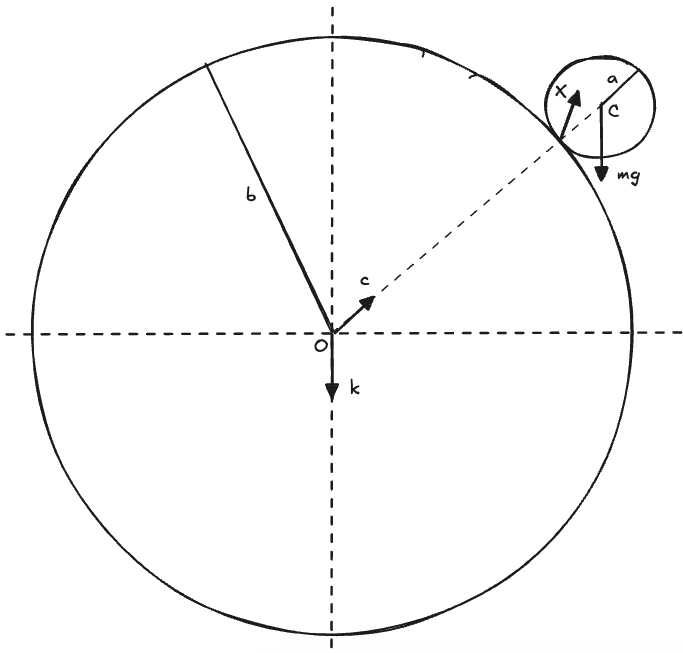
\includegraphics[scale=0.3]{ch19-3.png}
    \end{center}
    Then from the governing equations we have that
    \begin{align*}
        m\bm{\dot{V}} &= \bm{X} - mg\bm{k}\\
        \bm{\dot{L}}_C &= (-a\bm{c}) \times \bm{X} 
    \end{align*}
    Where $\bm{X}$ is the reaction of the sphere exerted on the ball.
    Using that $\bm{L}_C = A\bm{\omega}$ where $A = \frac{2}{5}ma^2$ is the
    moment of inertia of the ball and eliminating the reaction
    $\bm{X}$ we get that
    \begin{align*}
        A\bm{\dot{\omega}}
        &= (-a\bm{c}) \times (m\bm{\dot{V}} + mg\bm{k})\\
        &= a(m\bm{\dot{V}} + mg\uvk) \times \bm{c}\\
        &= ma(\bm{\dot{V}} \times \bm{c} + g\uvk \times \bm{c})
    \end{align*}
    Dot-multiplying the equation by $\bm{c}$ we obtain that
    \begin{align*}
        A\bm{c}\cdot\bm{\dot{\omega}}
        &= ma(\bm{c}\cdot(\bm{\dot{V}} \times \bm{c}) + g\bm{c}\cdot(\uvk \times \bm{c}))\\
        &= ma(0 + g\cdot 0)\\
        &= 0        
    \end{align*}
    If we now consider that the ball is rolling, then the particle in
    contact with the sphere has zero velocity, so the rolling condition give
    us
    \begin{align*}
        \bm{V} + a\bm{c} \times \bm{\omega} &= \bm{0}\\
        \bm{V} &= a\bm{\omega} \times \bm{c}
    \end{align*}
    Cross-multiplying this equation by $\bm{c}$ we get that
    \begin{align*}
        \bm{c} \times \bm{V} &= a\bm{c} \times (\bm{\omega} \times \bm{c})\\
        \bm{c} \times \bm{V} &= a(\bm{\omega} - (\bm{\omega} \cdot \bm{c})\bm{c})\\
        a\bm{\omega} &= (\bm{c} \times \bm{V}) + a(\bm{\omega} \cdot \bm{c})\bm{c}\\
        a\bm{\omega} &= (\bm{c} \times \bm{V}) + a\lambda\bm{c}
    \end{align*}
    Where $\lambda$ is a scalar function of time. 
    Also, we know that $\bm{V} = (a + b) \bm{\dot c}$ hence
    \begin{align*}
        a\bm{\omega} &= (a + b)\bm{c} \times \bm{\dot c} + a\lambda\bm{c}
    \end{align*}
    And derivating this equation we find that
    \begin{align*}
        a\bm{\dot \omega}
        &= (a + b)(\bm{\dot c} \times \bm{\dot c} + \bm{c} \times \bm{\ddot c})
        + a(\dot\lambda\bm{c} + \lambda\bm{\dot c})\\
        &= (a + b)\bm{c} \times \bm{\ddot c} + a(\dot\lambda\bm{c} + \lambda\bm{\dot c})
    \end{align*}
    Finally, dot-multypling this equation by $\bm{c}$ we obtain
    \begin{align*}
        a\bm{c}\cdot\bm{\dot \omega}
        &= (a + b)\bm{c}\cdot(\bm{c} \times \bm{\ddot c})
        + a\bm{c}\cdot(\dot\lambda\bm{c} + \lambda\bm{\dot c})\\
        0 &= 0 + a(\dot\lambda + 0)
    \end{align*}
    Therefore $\dot\lambda = 0$ which implies that
    $\lambda = \bm{\omega} \cdot \bm{c} = n$ where $n$ is constant.
    Which implies that the radial spin is conserved.

    On the other hand, by derivating the rolling condition we have that
    \begin{align*}
        \bm{\dot V}
        &= a\bm{\dot \omega} \times \bm{c} + a\bm{\omega} \times \bm{\dot c}
    \end{align*}
    Replacing these expressions and the value of $A$ in the equation for
    $A\bm{\dot\omega}$ we get that
    \begin{align*}
        \frac{2}{5}ma^2\bm{\dot{\omega}}
        &= ma(a(\bm{\dot \omega} \times \bm{c} + \bm{\omega} \times \bm{\dot c})
        \times \bm{c} + g\uvk \times \bm{c})\\
        2a\bm{\dot{\omega}}
        &= 5a(\bm{\dot \omega} \times \bm{c})\times\bm{c}
        + 5a(\bm{\omega} \times \bm{\dot c})\times \bm{c}
        + 5g\uvk \times \bm{c}\\
        2a\bm{\dot{\omega}}
        &= 5a(
            -(\bm{c}\cdot\bm{c})\bm{\dot \omega}
            + (\bm{c}\cdot\bm{\dot\omega})\bm{c}
        )
        + 5a(
            -(\bm{c}\cdot\bm{\dot c})\bm{\omega}
            + (\bm{c}\cdot\bm{\omega})\bm{\dot c}
        )
        + 5g\uvk \times \bm{c}\\
        2a\bm{\dot{\omega}}
        &= - 5a\bm{\dot \omega} + 0 - 0 + 5an\bm{\dot c} + 5g\uvk \times \bm{c}\\
        7a\bm{\dot{\omega}}
        &= 5an\bm{\dot c} + 5g\uvk \times \bm{c}\\
        7(a + b)\bm{c} \times \bm{\ddot c} + 2an\bm{\dot c}
        - 5g\uvk \times \bm{c} &= 0\\
        7(a + b)\bm{c} \times \bm{\ddot c} + 2an\bm{\dot c}
        + 5g\bm{c}\times\uvk &= 0
    \end{align*}
    Where we used that $\bm{c} \cdot \bm{c} = 1$, $\bm{c} \cdot \bm{\omega} = n$
    and $\bm{c} \cdot \bm{\dot c} = 0$.
    
    This equation matches with the equation of a spinning top which has a
    stable motion therefore the ball must have a stable motion too so it
    can roll on the spherical surface without ever falling off.

    Finally, at the highest point of the sphere the ball will be stable when 
    \begin{align*}
        C^2n^2 > 4Amgh
    \end{align*}
    Which is the equation that determines when a spinning top will be stable
    in the vertically upright position but we apply it to this case as follows
    \begin{align*}
        (2am)^2n^2 &> 4(7m(a + b))mg5 \\
        a^2n^2 &> 35g(a + b) \\
        n^2 &> \frac{35g(a + b)}{a^2}
    \end{align*}
\end{proof}
\cleardoublepage
\begin{proof}{\textbf{19.4}}
    We know that steady precession can only happen if 
    \begin{align*}
        A\cos\alpha \Omega^2 - C n \Omega + Mgh = 0
    \end{align*}
    In this case, since the axis of the top moves in the horizontal plane
    through $O$ we get that $\alpha = \pi/2$ and hence $\cos\alpha = 0$, then
    the equation becomes
    \begin{align*}
        - C n \Omega + Mgh = 0
    \end{align*}
    So there is only one rate of precession given by
    \begin{align*}
        \Omega = \frac{Mgh}{Cn}
    \end{align*}
\end{proof}
\cleardoublepage
\begin{proof}{\textbf{19.5}}
    We know the Lagrangian for the top is given by
    \begin{align*}
        L &= \frac{1}{2} A \dot\theta^2 + \frac{1}{2} A (\dot\phi\sin\theta)^2
        + \frac{1}{2}Cw+ \dot\phi\cos\theta)^2 - Mgh\cos\theta
    \end{align*}
    So the Lagrange equation for $\theta$ give us 
    \begin{align*}
        \derivative{}{t}\bigg(\partialderivative{L}{\dot\theta}\bigg) -
        \partialderivative{L}{\theta} = 0\\
        A\ddot\theta - A \dot\phi^2\sin\theta\cos\theta
        + C\dot\psi\dot\phi\sin\theta
        + C\dot\phi^2\sin\theta\cos\theta - Mgh\sin\theta
        = 0\\
        A\ddot\theta - A \dot\phi^2\sin\theta\cos\theta
        + C\dot\phi\sin\theta(\dot\psi
        + \dot\phi\cos\theta) - Mgh\sin\theta
        = 0
    \end{align*}
    Also, we know that
    \begin{align*}
        A\dot\phi\sin^2\theta + Cn\cos\theta
        &= L_z\\
        C(\dot\psi + \dot\phi\cos\theta) &= Cn
    \end{align*}
    But given that the top is spinning upright we see that $L_z = Cn$
    so we have that
    \begin{align*}
        A\dot\phi\sin^2\theta &= Cn(1 - \cos\theta)\\
        \dot\phi &= \frac{Cn(1 - \cos\theta)}{A\sin^2\theta}
    \end{align*}
    Replacing this value in the Lagrange equation we get that
    \begin{align*}
        A\ddot\theta - A \frac{C^2n^2(1 - \cos\theta)^2}{A^2 \sin^4\theta}
        \sin\theta\cos\theta
        + Cn\frac{Cn(1 - \cos\theta)}{A\sin^2\theta}\sin\theta - Mgh\sin\theta
        &= 0\\
        A\ddot\theta - \frac{C^2n^2(1 - \cos\theta)}{A \sin^2\theta}
        \bigg(
            \frac{(1 - \cos\theta)}{\sin^2\theta}\cos\theta
            - 1
        \bigg)\sin\theta
        - Mgh\sin\theta
        &= 0\\
        A\ddot\theta - \frac{C^2n^2(1 - \cos\theta)}{A \sin^2\theta}
        \bigg(
            \frac{\cos\theta - \cos^2\theta - \sin^2\theta}{\sin^2\theta}
        \bigg)\sin\theta
        - Mgh\sin\theta
        &= 0\\
        A\ddot\theta + \frac{C^2n^2(1 - \cos\theta)}{A \sin^2\theta}
        \bigg(\frac{1 - \cos\theta}{\sin^2\theta}\bigg)\sin\theta
        - Mgh\sin\theta
        &= 0\\
        A\ddot\theta + \frac{C^2n^2(1 - \cos\theta)^2}{A \sin^4\theta}
        \sin\theta - Mgh\sin\theta
        &= 0
    \end{align*}
    If we consider $\theta$ to be small we can approximate 
    $(1 - \cos\theta)^2/(\sin^4\theta)$ as 
    \begin{align*}
        \frac{(1 - \cos\theta)^2}{\sin^4\theta}
        &\approx \frac{(1 - (1 -\theta^2/2))^2}{\theta^4}
        = \frac{\theta^4/4}{\theta^4}
        = \frac{1}{4}
    \end{align*}
    Therefore, we can write that
    \begin{align*}
        A\ddot\theta + \bigg(\frac{C^2n^2}{4A} - Mgh\bigg)\theta &= 0
    \end{align*}
    Which is the equation for a Simple Harmonic Motion and hence for the motion
    to be stable it must happen that $\frac{C^2n^2}{4A} - Mgh$ is positive
    i.e.
    \begin{align*}
        C^2n^2 > 4AMgh
    \end{align*}
\end{proof}
\cleardoublepage
\begin{proof}{\textbf{19.6}}
    Given that a pencil is an axisymmetric body and we know from Problem 19.5
    that a body of this type will be stable in the upright position if
    \begin{align*}
        C^2n^2 > 4AMgh
    \end{align*}
    In this case we know that $C = \frac{1}{2}Mr^2$ and
    $A = \frac{1}{4}M r^2 + \frac{1}{12}M l^2 + \frac{Ml^2}{4}$ where $r$
    is the radius and $l$ is the length of the pencil.
    Also, we used the parallel axis theorem to determine $A$ with respect to
    $O$ and we assumed that the pencil is a uniform cylinder. Then
    \begin{align*}
        \bigg(\frac{1}{4}M^2r^4\bigg)n^2
        &> 4\bigg(\frac{1}{4}M r^2 + \frac{1}{12}M l^2 + \frac{Ml^2}{4}\bigg)Mgh\\
        \frac{1}{4}r^4n^2 &> gh\bigg(r^2 + \frac{1}{3}l^2 + l^2\bigg)\\
        n &> \sqrt{4gh\bigg(\frac{1}{r^2} + \frac{4l^2}{3r^4}\bigg)}
    \end{align*}
    Hence $n$ must be
    \begin{align*}
        n &> \sqrt{4\cdot 980~cm/s^2 \cdot 7.5~cm \cdot
        \bigg(\frac{1}{(0.35~cm)^2}
        + \frac{4 \cdot(15~cm)^2}{3\cdot(0.35~cm)^4}\bigg)}\\
        n &> 24248.61~rad/s
    \end{align*}
    Therefore for the pencil to remain stable in the upright position $n$ must
    be at least $3859.28~rev/s$

\end{proof}
\cleardoublepage
\begin{proof}{\textbf{19.7}}
\begin{itemize}
    \item [(i)] Taking the uniform solid ball as an axisymmetric body from
    Problem 19.5 we know that the ball can be stable rotating in the finger if
    \begin{align*}
        C^2n^2 > 4AMgh
    \end{align*}
    In this case we know we have that $C = \frac{2}{5}M(\frac{d}{2})^2$ and
    $A = \frac{2}{5}M (\frac{d}{2})^2 + M (\frac{d}{2})^2$ where $d$
    is the diameter of the ball.
    Also, we used the parallel axis theorem to determine $A$ with respect to
    $O$ which is where the ball touches the finger. Then
    \begin{align*}
        \bigg(\frac{1}{100}M^2d^4\bigg)n^2
        &> 4\bigg(\frac{1}{10}M d^2 + M \frac{d^2}{4}\bigg)Mgh\\
        \frac{1}{100}d^4n^2 &> gh\bigg(\frac{2}{5}d^2 + d^2\bigg)\\
        n &> \sqrt{140~\frac{gh}{d^2}}\\
        n &> \sqrt{70~\frac{g}{d}}
    \end{align*}
    Hence $n$ must be
    \begin{align*}
        n &> \sqrt{70\cdot\frac{980~cm/s^2}{20~cm}}\\
        n &> 58.56~rad/s
    \end{align*}
    Therefore for the uniform solid ball to remain stable $n$ must
    be at least $9.32~rev/s$.

    \item [(ii)] In the same way, for a uniform thin hollow ball, taking
    $C = \frac{2}{3}M(\frac{d}{2})^2$ and 
    $A = \frac{2}{3}M (\frac{d}{2})^2 + M (\frac{d}{2})^2$
    we have that 
    \begin{align*}
        \bigg(\frac{1}{36}M^2d^4\bigg)n^2
        &> 4\bigg(\frac{1}{6}M d^2 + M \frac{d^2}{4}\bigg)Mgh\\
        \frac{1}{36}d^4n^2 &> gh\bigg(\frac{2}{3}d^2 + d^2\bigg)\\
        n &> \sqrt{60~\frac{gh}{d^2}}\\
        n &> \sqrt{30~\frac{g}{d}}
    \end{align*}
    Hence $n$ must be
    \begin{align*}
        n &> \sqrt{30\cdot\frac{980~cm/s^2}{20~cm}}\\
        n &> 38.34~rad/s
    \end{align*}
    Therefore for the uniform thin hollow ball to remain stable $n$ must
    be at least $6.10~rev/s$.
\end{itemize}
Finally, given that most balls are not solid, the juggler should use the
determined $n$ for the uniform thin hollow ball.
\end{proof}
\cleardoublepage
\begin{proof}{\textbf{19.9}}
    From the equation of motion we see that
    \begin{align*}
        \bm{\dot{L}}_G &= -K\bm{\omega} 
    \end{align*}
    Where $K\bm{\omega}$ is the frictional couple.
    So from the equation of motion for a free axisymmetric body we have that
    \begin{align*}
        \frac{d}{dt}(A\bm{a}\times\bm{\dot a} + C\lambda\bm{a})
        &= -K\bm{\omega}\\
        A\bm{a}\times\bm{\ddot a} + C(\dot\lambda\bm{a} + \lambda\bm{\dot a})
        &= -K\bm{\omega}
    \end{align*}
    If we now take the scalar product of this equation with $\bm{a}$, we obtain
    \begin{align*}
        A\bm{a}\cdot(\bm{a}\times\bm{\ddot a})
        + C(\dot\lambda(\bm{a}\cdot \bm{a})
        + \lambda(\bm{a} \cdot \bm{\dot a}))
        &= -K\bm{a}\cdot \bm{\omega}\\
        C\dot\lambda &= -K\bm{a}\cdot \bm{\omega}\\
        \dot\lambda &= -\frac{K}{C}\lambda
    \end{align*}
    Then replacing this value of $\dot\lambda$ we get that 
    \begin{align*}
        A\bm{a}\times\bm{\ddot a} - K\lambda\bm{a} + C\lambda\bm{\dot a}
        &= -K\bm{\omega}\\
        A\bm{a}\times\bm{\ddot a}
        + K(\bm{\omega} - \lambda\bm{a})
        + C\lambda\bm{\dot a}
        &= 0
    \end{align*}
    But we know that the velocity of $\bm{a}$ is
    $\bm{\dot a} = \bm{\omega} \times \bm{a}$ and hence by taking the cross
    product of this equation with $\bm{a}$ we have that
    \begin{align*}
        \bm{a} \times \bm{\dot a} &= \bm{a} \times(\bm{\omega} \times \bm{a})\\
        &= (\bm{a} \cdot \bm{a})\bm{\omega} - (\bm{a}\cdot\bm{\omega})\bm{a}\\
        &= \bm{\omega} - \lambda \bm{a}
    \end{align*}
    Hence replacing this value we get that
    \begin{align*}
        A\bm{a}\times\bm{\ddot a}
        + K\bm{a}\times\bm{\dot a}
        + C\lambda\bm{\dot a}
        &= 0
    \end{align*}
    Taking the cross product of this equation with $\bm{\dot a}$ we get that
    \begin{align*}
        A\bm{\dot a}\times(\bm{a}\times\bm{\ddot a})
        + K\bm{\dot a}\times(\bm{a}\times\bm{\dot a})
        + C\lambda\bm{\dot a}\times\bm{\dot a}
        &= 0\\
        A((\bm{\dot a} \cdot \bm{\ddot a})\bm{a} - (\bm{\dot a} \cdot \bm{a})\bm{\ddot a}) 
        + K((\bm{\dot a} \cdot \bm{\dot a})\bm{a} - (\bm{\dot a} \cdot \bm{a})\bm{a})
        &= 0\\
        A(\bm{\dot a} \cdot \bm{\ddot a})\bm{a} + K|\bm{\dot a}|^2\bm{a} &= 0\\
        A\bm{\dot a} \cdot \bm{\ddot a} + K|\bm{\dot a}|^2 &= 0
    \end{align*}
    But also we know that
    \begin{align*}
        \frac{d}{dt}|\bm{\dot a}|^2
        = \frac{d}{dt}(\bm{\dot a} \cdot \bm{\dot a})
        &= \bm{\ddot a} \cdot \bm{\dot a} + \bm{\dot a} \cdot \bm{\ddot a}
        = 2\bm{\dot a} \cdot \bm{\ddot a}
    \end{align*}
    Hence
    \begin{align*}
        A\frac{d}{dt}|\bm{\dot a}|^2 + 2K|\bm{\dot a}|^2 &= 0
    \end{align*}
    The solution to this differential equation gives us
    \begin{align*}
        |\bm{\dot a}| &= \frac{A}{2K}De^{-\frac{K}{A}t}
    \end{align*}
    Where $D$ is a constant.

    Finally, to determine the angle $\theta$ between $\bm\omega$ and $\bm{a}$
    we can compute $\tan\theta$ as follows
    \begin{align*}
        \tan\theta
        = \frac{\sin\theta}{\cos\theta}
        = \frac{|\bm{\omega}||\bm{a}|\sin\theta}{|\bm{\omega}||\bm{a}|\cos\theta}
        = \frac{|\bm{\omega}\times \bm{a}|}{\bm{\omega}\cdot\bm{a}}
        = \frac{|\bm{\dot a}|}{\lambda}
    \end{align*}
    So we need an equation to determine $\lambda$. By solving the equation
    $\dot\lambda + \frac{K}{C}\lambda = 0$ which we derived above we get that
    \begin{align*}
        \lambda = Ee^{-\frac{K}{C}t}    
    \end{align*}
    Where $E$ is another constant.
    Then
    \begin{align*}
        \tan\theta
        &= \frac{ADe^{-\frac{K}{A}t}}{2KEe^{-\frac{K}{C}t}}\\
        \tan\theta
        &= \frac{AD}{2KE}e^{(\frac{K}{C}-\frac{K}{A})t}\\
        \theta
        &= \arctan\bigg(\frac{AD}{2KE}e^{K(\frac{1}{C}-\frac{1}{A})t}\bigg)
    \end{align*}
    Hence if $C > A$ the function $e^{K(\frac{1}{C}-\frac{1}{A})t}$ decreases
    with time and therefore $\theta$ decreases.
\end{proof}
\cleardoublepage
\begin{proof}{\textbf{19.10}}
    Let us consider a spinning hoop as shown below
    \begin{center}
        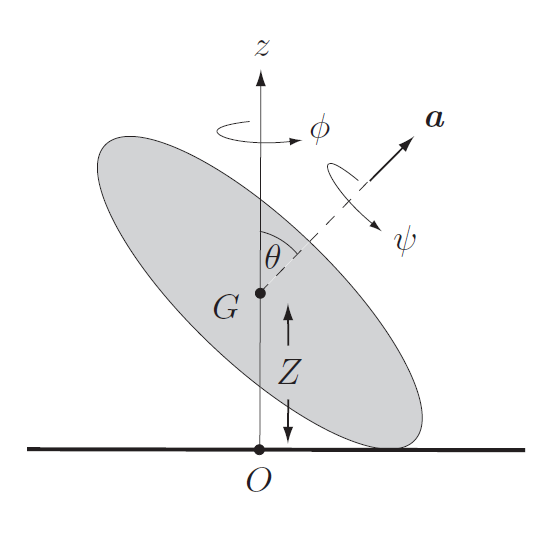
\includegraphics[scale=0.45]{ch19-10.png}
    \end{center}
    The kinetic energy in terms of the Euler angles is
    \begin{align*}
        T = \frac{1}{2}M\dot Z^2 + \frac{1}{2}A\dot\theta^2
        + \frac{1}{2}A(\dot\phi\sin\theta)^2
        + \frac{1}{2}C(\dot\psi + \dot\phi\cos\theta)^2
    \end{align*}
    Where $A$ and $C$ are the principal moments of inertia with respect to $G$.
    By geometry we see that
    \begin{align*}
        Z = a \sin\theta
    \end{align*}
    and hence $\dot Z = a\dot\theta \cos\theta$ so the kinetic energy becomes
    \begin{align*}
        T &= \frac{1}{2}M(a\dot\theta \cos\theta)^2
        + \frac{1}{2}A\dot\theta^2
        + \frac{1}{2}A(\dot\phi\sin\theta)^2
        + \frac{1}{2}C(\dot\psi + \dot\phi\cos\theta)^2\\
        &= \frac{1}{2}\dot\theta^2 (Ma^2\cos^2\theta + A)
        + \frac{1}{2}A(\dot\phi\sin\theta)^2
        + \frac{1}{2}C(\dot\psi + \dot\phi\cos\theta)^2
    \end{align*}
    Also, the gravitational potential energy is given by
    \begin{align*}
        V = MgZ = Mga\sin\theta
    \end{align*}
    Then the Lagrangian for the spinning hoop is
    \begin{align*}
        L =  \frac{1}{2}\dot\theta^2 (Ma^2\cos^2\theta + A)
        + \frac{1}{2}A(\dot\phi\sin\theta)^2
        + \frac{1}{2}C(\dot\psi + \dot\phi\cos\theta)^2 - Mga\sin\theta
    \end{align*}
    Since the Lagrangian doesn't depend on $\phi$ or $\psi$
    then the generalized momenta $p_\phi$ and $p_\psi$ are conserved. Hence
    \begin{align*}
        A\dot\phi\sin^2\theta + C(\dot\psi + \dot\phi\cos\theta)\cos\theta
        &= L_z\\
        C(\dot\psi + \dot\phi\cos\theta) &= Cn
    \end{align*}
    Where $L_z$ and $n$ are constants.
    Let us compute now the Lagrange equation for $\theta$, i.e.
    \begin{align*}
        \derivative{}{t}\partialderivative{L}{\dot\theta}
        - \partialderivative{L}{\theta} = 0
    \end{align*}
    Hence
    \begin{align*}
        &\derivative{}{t}[\dot\theta(Ma^2\cos^2\theta + A)]
        - [-\dot\theta^2 Ma^2\sin\theta\cos\theta
        + A\dot\phi^2\sin\theta\cos\theta
        - C\dot\psi\dot\phi\sin\theta\\
        &\quad - C\dot\phi^2\sin\theta\cos\theta - Mga\cos\theta] = 0\\
        &\derivative{}{t}[\dot\theta(Ma^2\cos^2\theta + A)]
        + [\dot\theta^2 Ma^2\sin\theta\cos\theta
        - A\dot\phi^2\sin\theta\cos\theta\\
        &\quad+ Cn\dot\phi\sin\theta + Mga\cos\theta] = 0
    \end{align*}
    If we consider that the angle between the hoop and the floor is a constant
    $\alpha$ and we assume that $\Omega$ is the rate of steady precession
    the Lagrange equation for $\theta$ becomes
    \begin{align*}
        -A\Omega^2\sin\alpha\cos\alpha + Cn\Omega\sin\alpha + Mga\cos\alpha &= 0        
    \end{align*}
    Now by replacing the values of $A = 1/2Ma^2$ and $C = Ma^2$ we get that
    \begin{align*}
        -\frac{1}{2}Ma^2\Omega^2\sin\alpha\cos\alpha
        + Ma^2n\Omega\sin\alpha + Mga\cos\alpha &= 0\\
        -\Omega^2\sin\alpha\cos\alpha
        + 2n\Omega\sin\alpha + 2\frac{g}{a}\cos\alpha &= 0\\
        \Omega^2\cos\alpha - 2n\Omega - 2\frac{g}{a}\cot\alpha &= 0
    \end{align*}
    The solution to this equation in terms of $\Omega$ is
    \begin{align*}
        \Omega &= \frac{2n \pm \sqrt{4n^2 + 8g\cos\alpha\cot\alpha/a}}{2\cos\alpha}\\
        &= \frac{2n}{2\cos\alpha}
        \bigg(1 \pm \sqrt{1 + \frac{8g\cos\alpha\cot\alpha}{4an^2}}\bigg)
    \end{align*}
    If we assume that $8g\cos\alpha\cot\alpha/4an^2$ is small we can apply the
    binomial approximation as follows
    \begin{align*}
        \Omega &= \frac{n}{\cos\alpha}
        \bigg(1 \pm \bigg(1 + \frac{g\cos\alpha\cot\alpha}{an^2}\bigg)\bigg)
    \end{align*}
    So the fast and slow solutions for the precession $\Omega$ are
    \begin{align*}
        \Omega^F &= \frac{n}{\cos\alpha}
        \bigg(2 + \frac{g\cos\alpha\cot\alpha}{an^2}\bigg)
        = \frac{2n}{\cos\alpha} + \frac{g\cot\alpha}{an}\\
        \Omega^S &= \frac{n}{\cos\alpha}
        \bigg(-\frac{g\cos\alpha\cot\alpha}{an^2}\bigg)
        = -\frac{g\cot\alpha}{an}
    \end{align*}
    Where the fast precession goes in the "same way" as $n$ and the slower one
    goes in the "opposite direction" (because of the minus sign).
\end{proof}
\cleardoublepage
\begin{proof}{\textbf{19.12}}
    Let an unsymmetrical body to be in steady rotation about the principal
    axis $Gx_1$ through $G$ and suppose we disturb the body slightly.
    In the initial motion we can assume that $\omega_2 = \omega_3 = 0$
    and $\omega_1 = \Lambda$ for some $\Lambda$ constant.
    But after some small disturbance we get that  
    $\omega_1 = \Lambda + a_1$ and that $\omega_2$ and $\omega_3$ are small
    but not zero.
 
    The Euler's equations state the following
    \begin{align*}
        A\dot\omega_1 - (B - C)\omega_2\omega_3 &= 0\\
        B\dot\omega_2 - (C - A)\omega_3\omega_1 &= 0\\
        C\dot\omega_3 - (A - B)\omega_1\omega_2 &= 0
    \end{align*}
    After linealization and taking into account the variation of 
    $\omega_1$ we get that
    \begin{align*}
        A\dot{a}_1 &= 0\\
        B\dot\omega_2 - (C - A)(\Lambda + a_1)\omega_3 &= 0\\
        C\dot\omega_3 - (A - B)(\Lambda + a_1)\omega_2 &= 0
    \end{align*}
    But given that $a_1$ is a small variation and $\omega_3$ and $\omega_2$
    are small too, we can drop the products to get the following
    \begin{align*}
        A\dot{\omega}_1 &= 0\\
        B\dot\omega_2 - (C - A)\Lambda\omega_3 &= 0\\
        C\dot\omega_3 - (A - B)\Lambda\omega_2 &= 0
    \end{align*}
    Where we wrote back that $\dot\omega_1 = \dot a_1$. Derivating the second
    equation we get that
    \begin{align*}
        B\ddot\omega_2 - (C - A)\Lambda\dot\omega_3 &= 0
    \end{align*}
    And replacing $\dot\omega_3$ from the third equation we get that 
    \begin{align*}
        B\ddot\omega_2 - (C - A)\Lambda\frac{(A - B)}{C}\Lambda\omega_2 &= 0\\
        \ddot\omega_2 + \frac{(A - C)(A - B)}{BC}\Lambda^2\omega_2 &= 0
    \end{align*}
    This is the equation for a Simple Harmonic Motion and hence for the motion
    to be stable it must happen that
    \begin{align*}
        \frac{(A - C)(A - B)}{BC}\Lambda^2 > 0
    \end{align*} 
    Therefore must be that $A > C$ and $A > B$ or $A < C$ and $A < B$ i.e.
    $A$ is the largest or smallest moment of inertia.

    Doing the same for $\omega_3$ we get that
    \begin{align*}
        C\ddot\omega_3 - (A - B)\Lambda\frac{(C - A)}{B}\Lambda\omega_2 &= 0\\
        \ddot\omega_2 + \frac{(A - C)(A - B)}{BC}\Lambda^2\omega_2 &= 0
    \end{align*}
    Which tells us the same restrictions about $A$ i.e. $A$ is the largest or
    smallest moment of inertia.

    We could do the same perturbation analysis for $\omega_2$ and $\omega_3$
    but the analysis is analogous and we will get that for the unsymmetrical
    body to be stable while rotating about $Gx_2$ we need that $B$ to be the
    largest or smallest moment of inertia.
    The same is true for when the body is rotating about $Gx_3$ and the moment
    of inertia $C$ needs to be the largest or smallest.
\end{proof}
\cleardoublepage
\begin{proof}{\textbf{19.13}}
    Given that the Frisbee is an axisymmetric body the Euler's equations
    become
    \begin{align*}
        A\dot\omega_1 - (A - C)\omega_2\omega_3 &= -K \omega_1\\
        A\dot\omega_2 - (C - A)\omega_3\omega_1 &= -K \omega_2\\
        C\dot\omega_3 &= -K \omega_3
    \end{align*}
    From the third equation we have that
    \begin{align*}
        \omega_3 &= C_1 e^{-\frac{K}{C} t}
    \end{align*}
    Where $C_1$ is a constant.
    Multiplying the first equiation by $\omega_1$ and the second by $\omega_2$
    we get that
    \begin{align*}
        A\dot\omega_1\omega_1 - (A - C)\omega_3\omega_2\omega_1
        &= -K \omega_1^2\\
        A\dot\omega_2\omega_2 + (A - C)\omega_3\omega_2\omega_1
        &= -K \omega_2^2
    \end{align*}
    Now we sum both equations
    \begin{align*}
        -K \omega_1^2 -K \omega_2^2
        &= A\dot\omega_1\omega_1 + A\dot\omega_2\omega_2\\
        \omega_1^2 + \omega_2^2
        &= -\frac{A}{K}(\dot\omega_1\omega_1 + \dot\omega_2\omega_2)
    \end{align*}
    Let us note that
    \begin{align*}
        \frac{d}{dt}(\omega_1^2 + \omega_2^2)
        = 2(\dot\omega_1\omega_1 + \dot\omega_2\omega_2)
    \end{align*}
    So we can write the differential equation as
    \begin{align*}
        \frac{d}{dt}(\omega_1^2 + \omega_2^2) 
        + 2\frac{K}{A}(\omega_1^2 + \omega_2^2) = 0
    \end{align*}
    The solution to this equation is
    \begin{align*}
        \omega_1^2 + \omega_2^2 = C_2e^{- 2\frac{K}{A}t}
    \end{align*}
    To compute the angle $\theta$ between $\bm\omega$ and $\bm a$ we follow
    the same procedure as before. Let us observe that in this case, the unit
    vector $\bm{a}$ is in the direction of $\omega_3$ then
    \begin{align*}
        \tan\theta
        &= \frac{|\bm{\omega} \times \bm{a}|}{\bm{\omega} \cdot \bm{a}}\\
        \tan\theta
        &= \frac{\sqrt{(\omega_2 a_3)^2 + (-\omega_1 a_3)^2}}{\omega_3}\\
        \tan\theta
        &= \frac{\sqrt{C_2e^{- 2\frac{K}{A}t}}}{C_1 e^{-\frac{K}{C} t}}\\
        \theta &= \arctan(C_3e^{K(\frac{1}{C}-\frac{1}{A})t})
    \end{align*}
    Where $C_3$ is another constant.
    Hence if $C > A$ the function $e^{K(\frac{1}{C}-\frac{1}{A})t}$ decreases
    with time and therefore $\theta$ decreases.
\end{proof}
\cleardoublepage
\begin{proof}{\textbf{19.16}}
    We know that the Lagrangian of the top is
    \begin{align*}
        L = \frac{1}{2}A\dot\theta^2 + \frac{1}{2}A(\dot\phi\sin\theta)^2
        + \frac{1}{2}C(\dot\psi + \dot\phi\cos\theta)^2 - Mgh\cos\theta
    \end{align*}
    Then the Lagrange's equation for $\theta$ is
    \begin{align*}
        \derivative{}{t}\bigg(\partialderivative{L}{\dot\theta}\bigg)
        - \partialderivative{L}{\theta} = 0\\
        A\ddot\theta
        - \bigg[A\dot\phi^2\sin\theta\cos\theta
        + C(-\dot\psi\dot\phi\sin\theta - \dot\phi^2\sin\theta\cos\theta)
        + Mgh\sin\theta\bigg] = 0\\
        A\ddot\theta
        - A\dot\phi^2\sin\theta\cos\theta
        + C(\dot\psi\dot\phi\sin\theta + \dot\phi^2\sin\theta\cos\theta)
        - Mgh\sin\theta = 0
    \end{align*}
    For $\phi$ we have that
    \begin{align*}
        \derivative{}{t}\bigg(\partialderivative{L}{\dot\phi}\bigg)
        - \partialderivative{L}{\phi} &= 0\\
        \frac{d}{dt}
        (A\dot\phi\sin^2\theta + C(\dot\psi\cos\theta + \dot\phi\cos^2\theta))
        &= 0\\
        A(\ddot\phi\sin^2\theta + 2\dot\phi\dot\theta\sin\theta\cos\theta)
        + C(\ddot\psi\cos\theta - \dot\psi\dot\theta\sin\theta
        + \ddot\phi\cos^2\theta&\\
        - 2\dot\phi\dot\theta\sin\theta\cos\theta) &= 0
    \end{align*}
    And for $\psi$ we get that
    \begin{align*}
        \derivative{}{t}\bigg(\partialderivative{L}{\dot\psi}\bigg)
        - \partialderivative{L}{\psi} &= 0\\
        \frac{d}{dt}(C(\dot\psi + \dot\phi\cos\theta)) &= 0\\
        C(\ddot\psi + \ddot\phi\cos\theta - \dot\phi\dot\theta\sin\theta) &= 0
    \end{align*}
    Let us name $\dot\theta = u$, $\dot\phi = v$ and $\dot\psi = w$ then
    we can write the equation for $\theta$ as
    \begin{align*}
        \dot u &= 
        v^2\sin\theta\cos\theta
        - \frac{C}{A}(wv\sin\theta + v^2\sin\theta\cos\theta)
        + \frac{Mgh}{A}\sin\theta
    \end{align*}
    We can write the equation for $\psi$ as
    \begin{align*}
        C(\dot{w} + \dot{v}\cos\theta - vu\sin\theta) &= 0\\
        C(\dot{w}\cos\theta + \dot{v}\cos^2\theta - vu\sin\theta\cos\theta) &= 0
    \end{align*}
    Where we multiplied by $\cos\theta$ in the end so we can subtract it from
    the equation for $\phi$ which states the following
    \begin{align*}
        &A(\dot v\sin^2\theta + 2vu\sin\theta\cos\theta)
        + C(\dot{w}\cos\theta - wu\sin\theta
        + \dot{v}\cos^2\theta\\
        &- 2vu\sin\theta\cos\theta) = 0
    \end{align*}
    hence subracting them we get that
    \begin{align*}
        A(\dot v\sin^2\theta + 2vu\sin\theta\cos\theta)
        - C(wu\sin\theta + vu\sin\theta\cos\theta) &= 0
    \end{align*}
    Which implies that
    \begin{align*}
        \dot v &= \frac{
            C/A(wu\sin\theta + vu\sin\theta\cos\theta)
        - 2vu\sin\theta\cos\theta}{\sin^2\theta}
    \end{align*}
    Finally we can replace this value in the equation for $\psi$ to get
    an equation for $\dot{w}$ as follows
    \begin{align*}
        \dot{w} &= vu\sin\theta - \frac{
            C/A(wu\sin\theta + vu\sin\theta\cos\theta)
        - 2vu\sin\theta\cos\theta}{\sin^2\theta}\cos\theta
    \end{align*}
    Now we can solve the system of first-order differential equations
    using the Runge-Kutta method.
    Below we show some results
    \begin{center}
        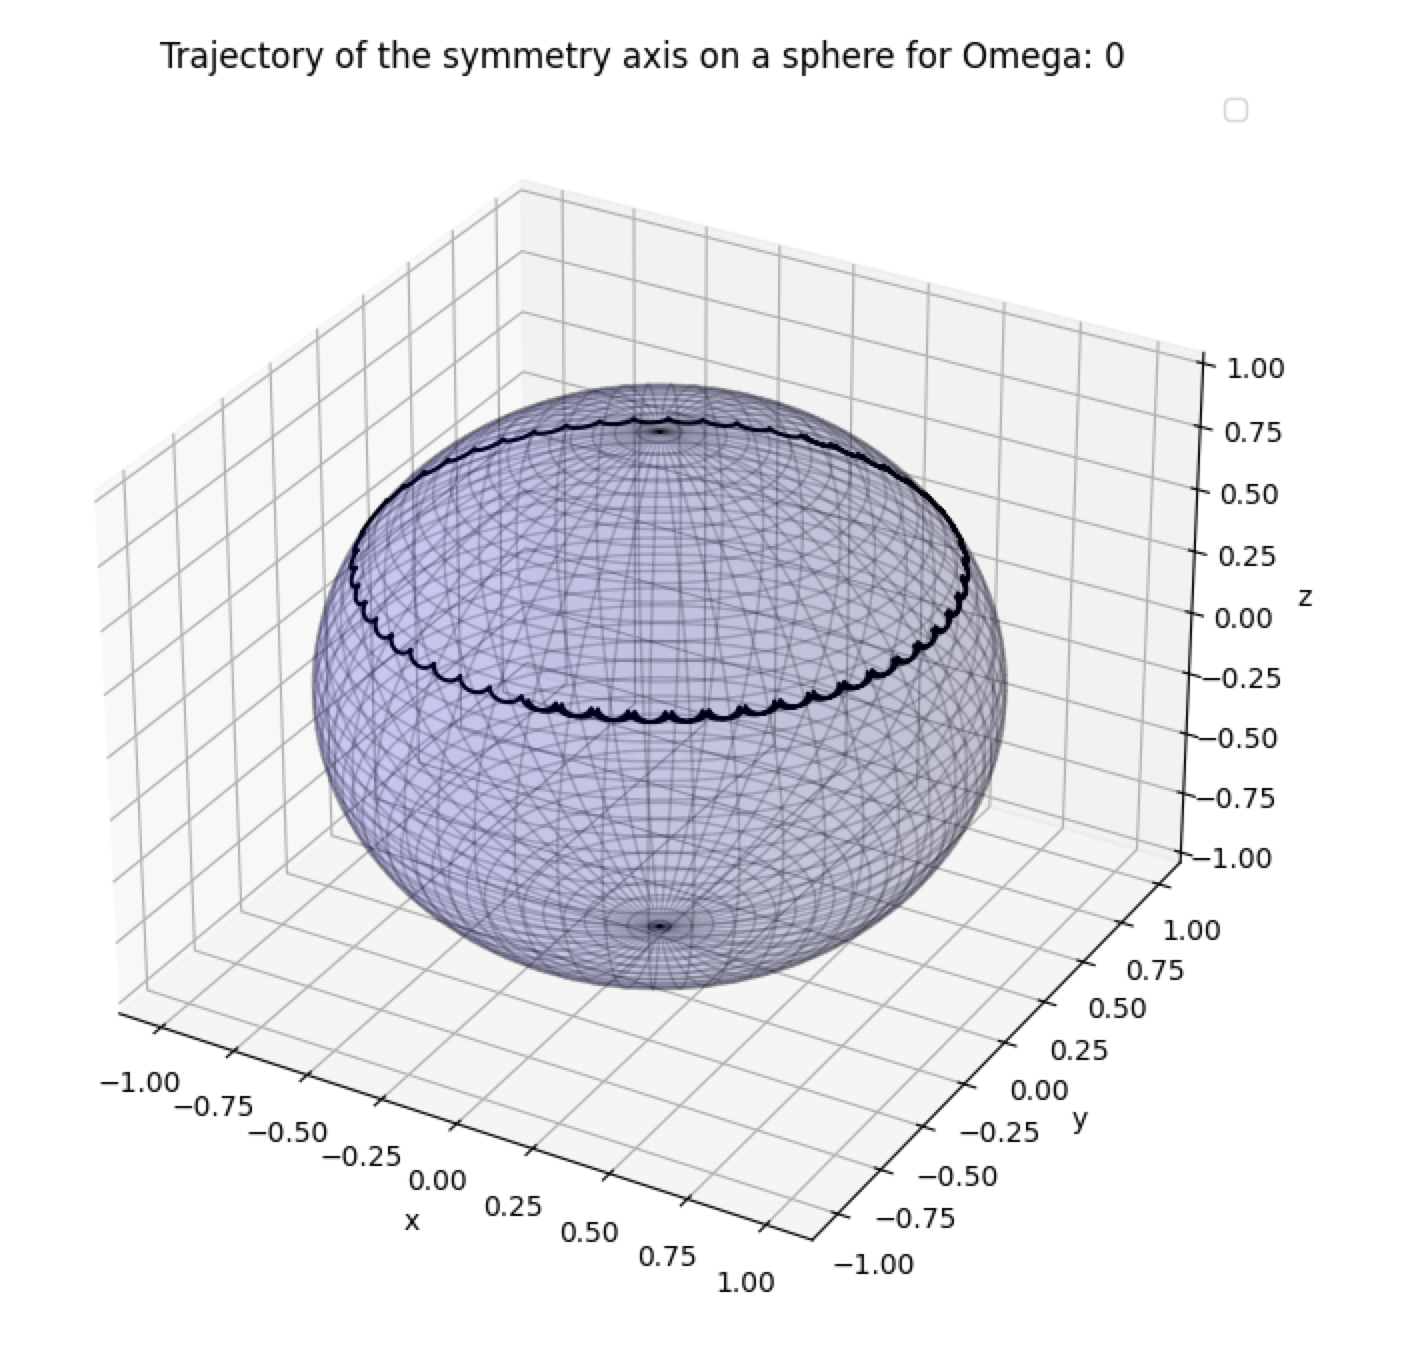
\includegraphics[scale=0.4]{ch19-16-1.png}
        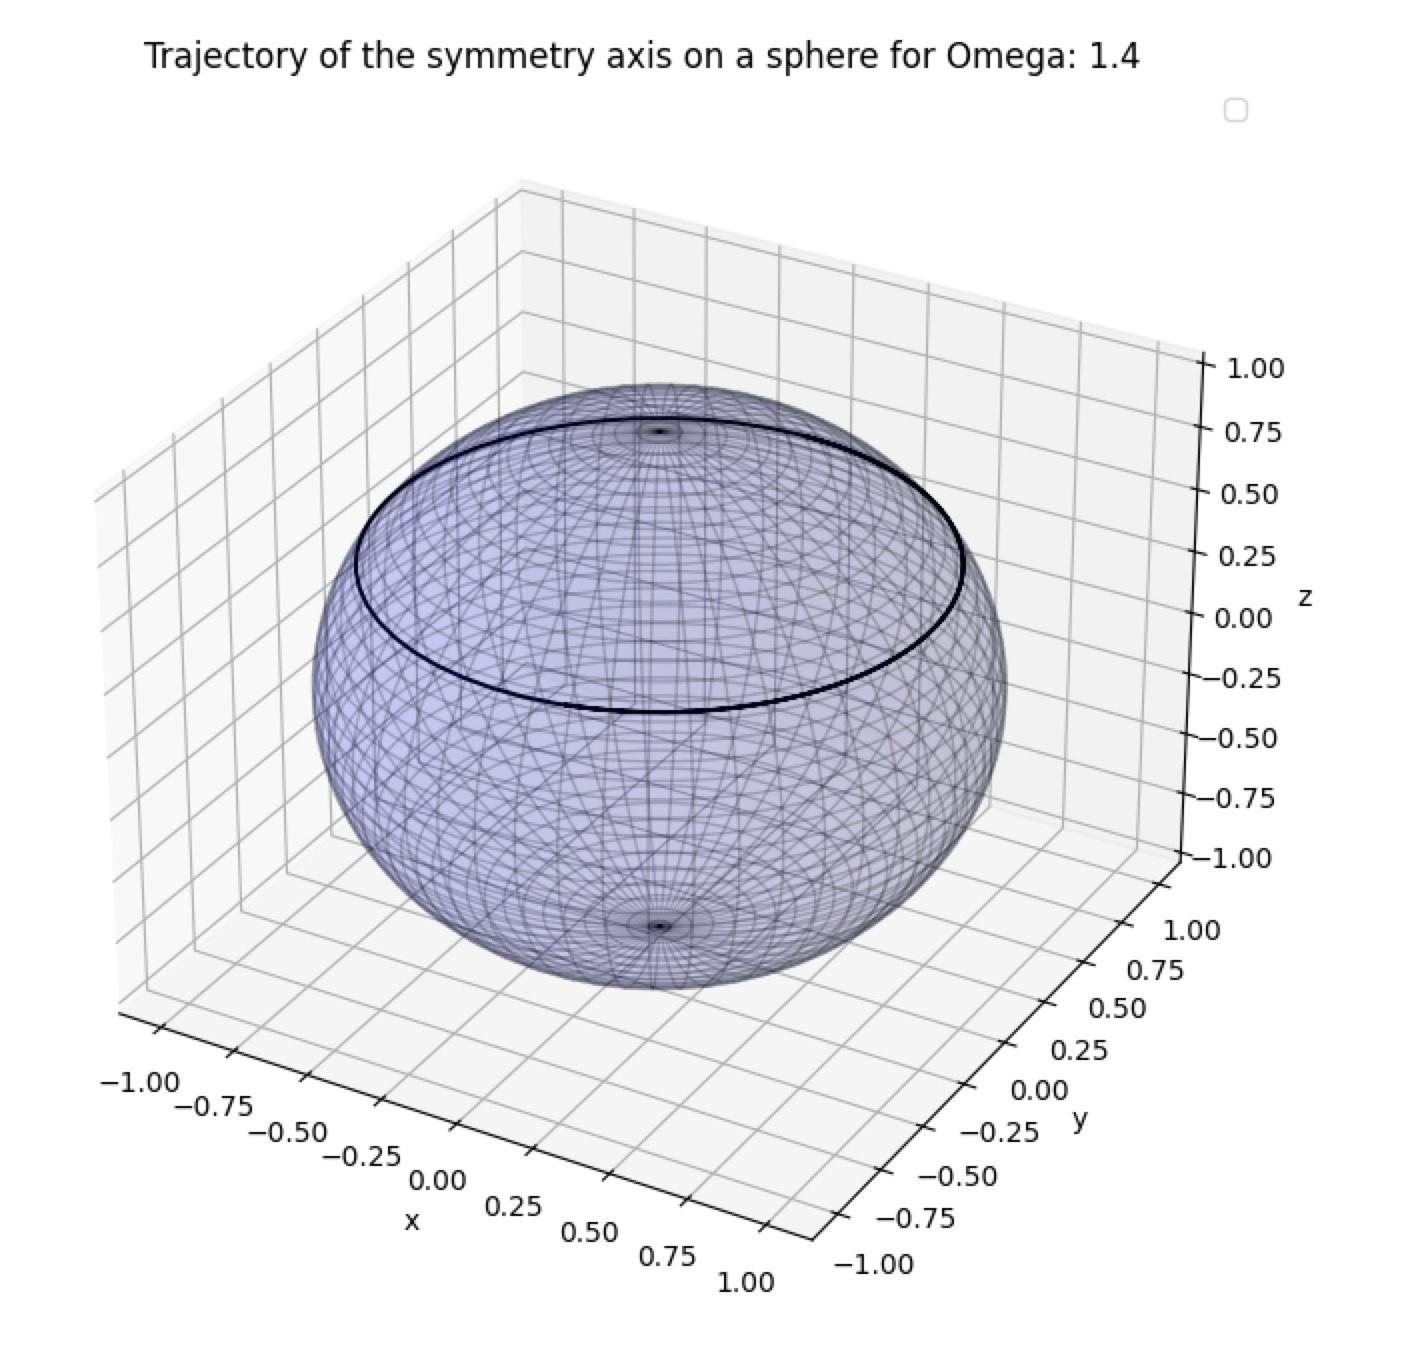
\includegraphics[scale=0.4]{ch19-16-2.png}
        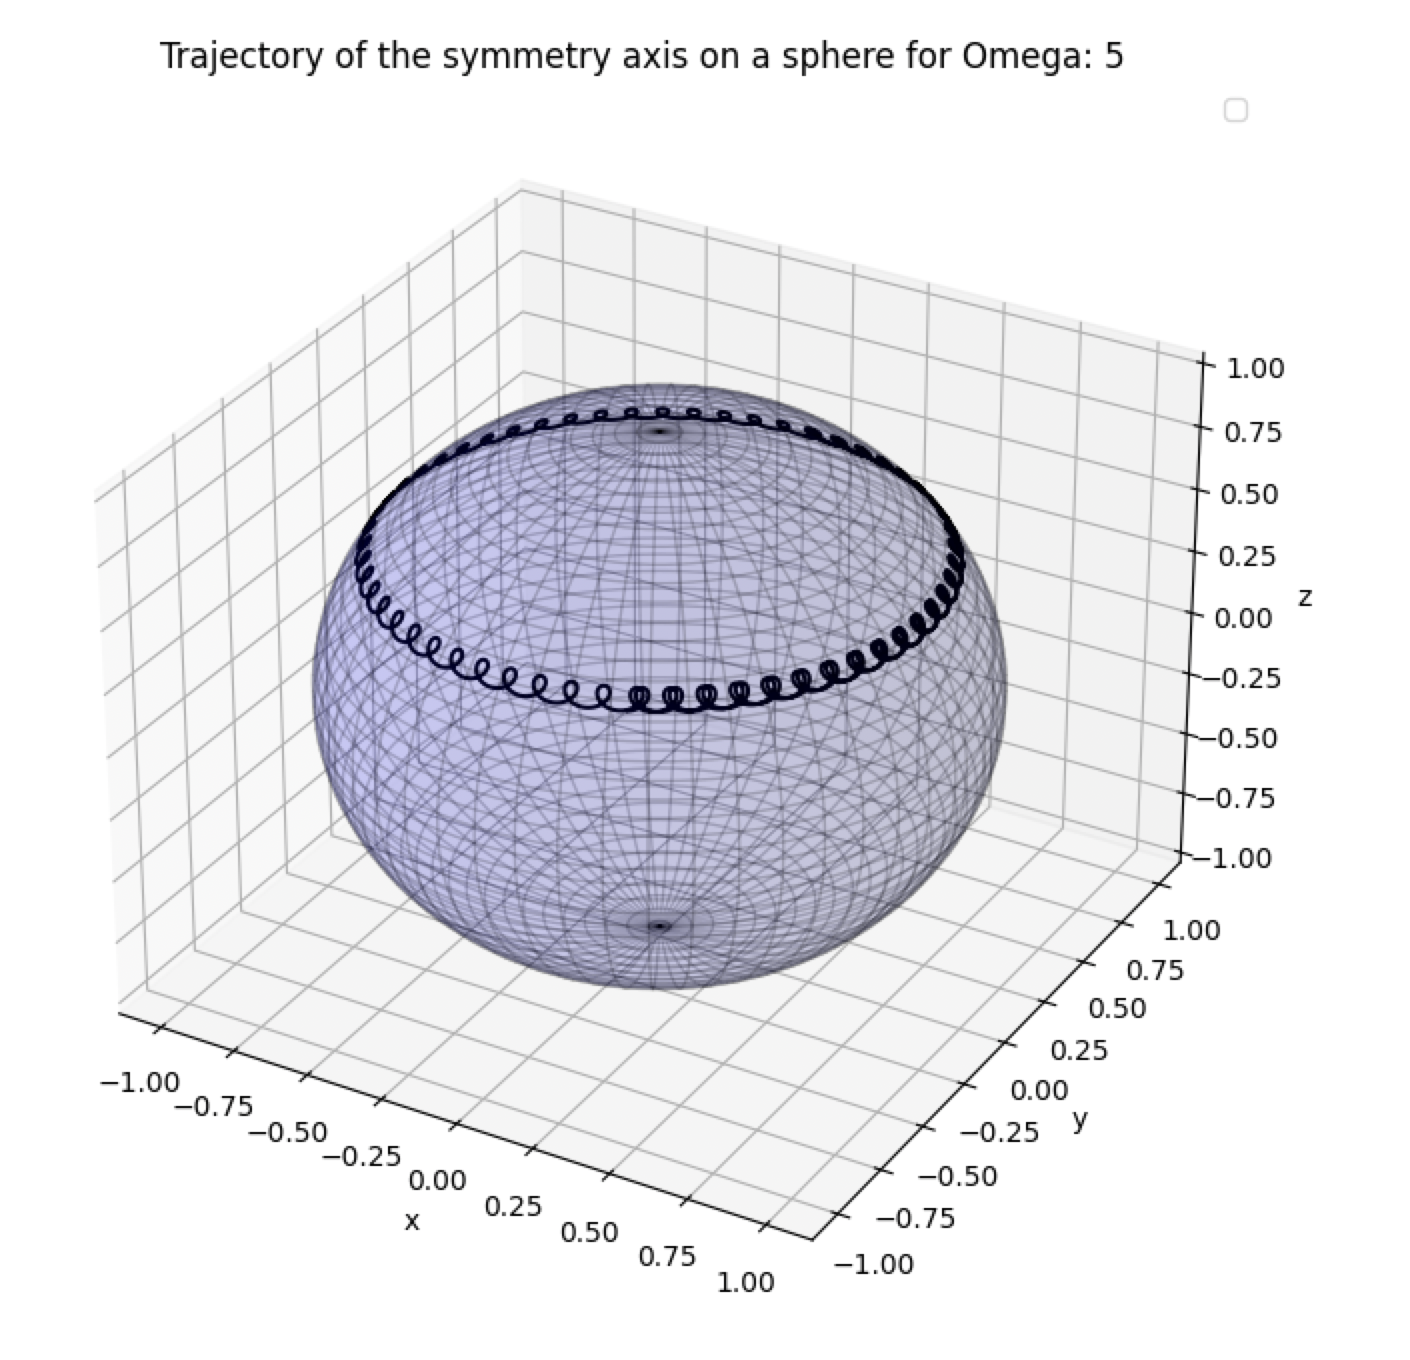
\includegraphics[scale=0.4]{ch19-16-3.png}
        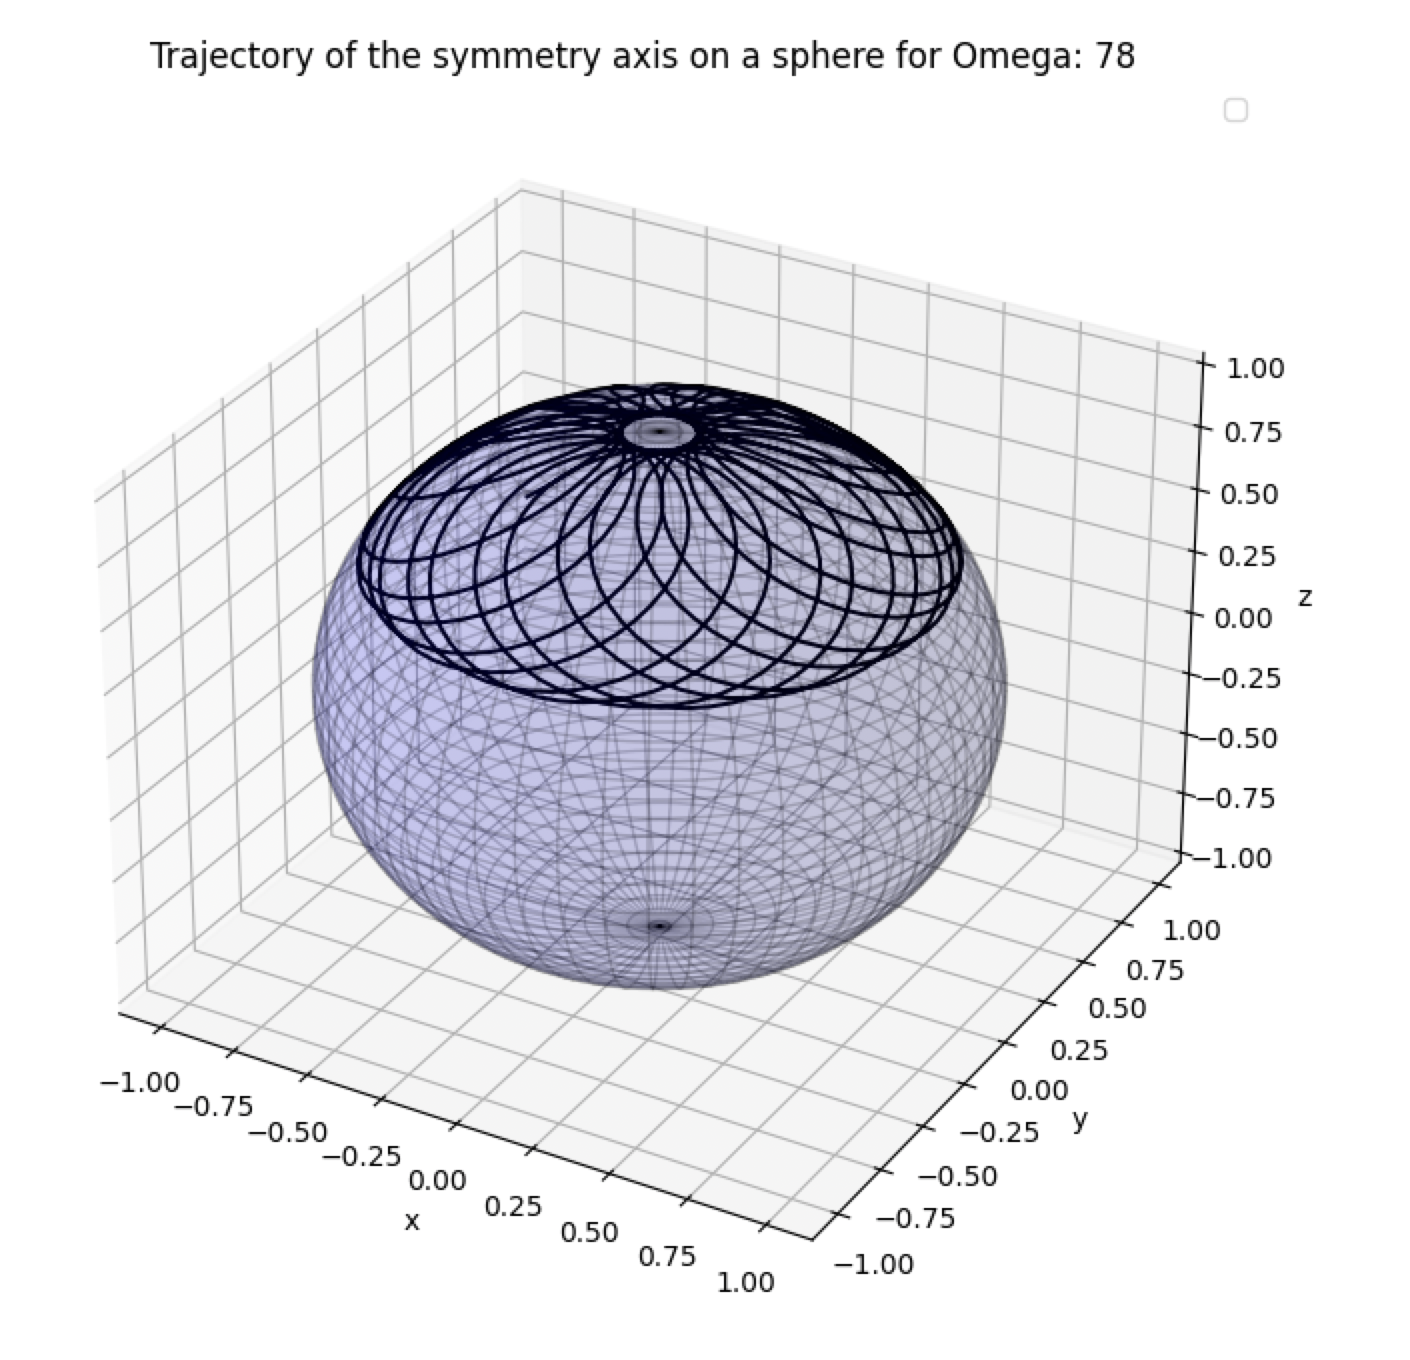
\includegraphics[scale=0.4]{ch19-16-4.png}
    \end{center}
\end{proof}
\cleardoublepage
\begin{proof}{\textbf{19.17}}
    We want to obtain the paths of the $\bm L$-point for an unsymmetrical body.
    Euler equations in terms of the components of $\bm{L}$ in the frame
    $Gxyz$ give us the following 
    \begin{align*}
        \dot{L}_x &= \frac{(B - C)}{BC}L_yL_z\\
        \dot{L}_y &= \frac{(C - A)}{AC}L_zL_x\\
        \dot{L}_z &= \frac{(A - B)}{AB}L_xL_y
    \end{align*}
    Also, the equations for $\bm{\dot{e}_1}$, $\bm{\dot{e}_2}$ and
    $\bm{\dot{e}_3}$ gives us    
    \begin{equation*}
    \begin{aligned}
        \dot{e}_{1x} &= 0\\
        \dot{e}_{1y} &= \omega_z = \frac{L_z}{C}\\
        \dot{e}_{1z} &= -\omega_y = -\frac{L_y}{B}
    \end{aligned}
    \qquad
    \begin{aligned}
        \dot{e}_{2x} &= -\omega_z = -\frac{L_z}{C}\\
        \dot{e}_{2y} &=  0\\ 
        \dot{e}_{2z} &= \omega_x = \frac{L_x}{A}
    \end{aligned}
    \qquad
    \begin{aligned}
        \dot{e}_{3x} &= \omega_y = \frac{L_y}{B}\\
        \dot{e}_{3y} &= -\omega_x = -\frac{L_x}{A}\\
        \dot{e}_{3z} &= 0
    \end{aligned}
    \end{equation*}
    Finally, we can solve the system of twelve first-order differential
    equations using the Runge-Kutta method.
    Below we show the result
    \begin{center}
        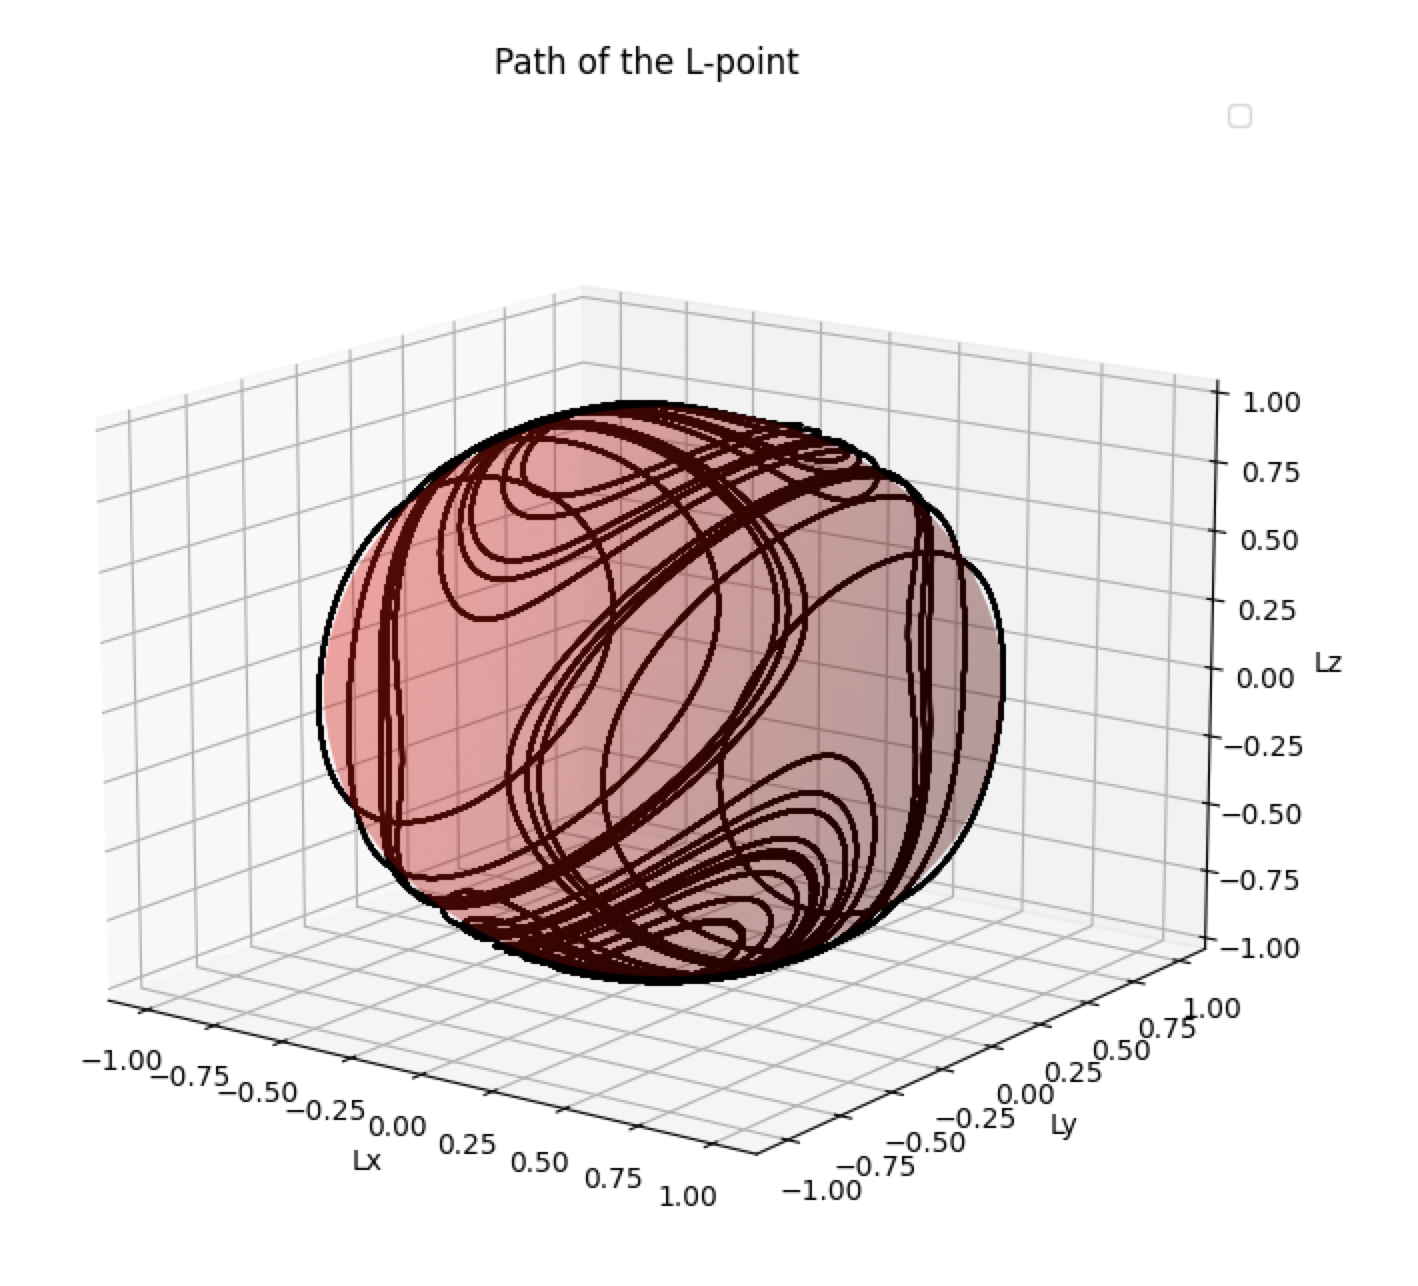
\includegraphics[scale=0.4]{ch19-17.png}
    \end{center}
\end{proof}

\end{document}

















